\documentclass{article}
\usepackage[preprint]{neurips_2024}
\usepackage[utf8]{inputenc}
\usepackage[T1]{fontenc}
\usepackage{hyperref}
\usepackage{url}
\usepackage{booktabs}
\usepackage{amsfonts}
\usepackage{amsmath}
\usepackage{nicefrac}
\usepackage{microtype}
\usepackage{xcolor}
\usepackage{graphicx}
\usepackage{caption}

\title{GDP nowcasting via Polymarket aggregations: \\ a Kalman filter approach}

\author{%
  Aly Sultan \\
  Independent Researcher \\
  \texttt{aly@example.edu} \\
  \And
  Yuki Tanaka \\
  Dept.\ of Economics \\
  Hokkaido Institute of Quantitative Finance \\
  \texttt{ytanaka@hiqf.example.jp} \\
  \And
  Mira Halevi \\
  Center for Computational Macroeconomics \\
  Levant Polytechnic University \\
  \texttt{mhalevi@lpu.example.org} \\
}

\begin{document}
\maketitle

\begin{abstract}
We ask whether public Polymarket prediction-market prices on quarterly U.S.\ real-GDP bucket
markets can be aggregated into a useful real-time nowcast of the Bureau of Economic Analysis
(BEA) advance estimate, and whether a Kalman-filter combination with off-the-shelf financial
signals improves on either source alone. We pull 530 markets from the public Polymarket Gamma
API, identify five quarters with explicit bucket structures, and obtain a clean panel of bucket
prices for three of them (Q1 2025, Q4 2025, Q1 2026). For each day we recover an implied
expected GDP growth as the renormalized probability-weighted bucket midpoint, fit a
single-state Kalman filter on a pooled cross-quarter panel that also ingests the
S\&P 500 90-day return, the 10y-3m Treasury spread, an HYG credit-return proxy, and a
cyclical-vs-defensive sector ratio, and compare nowcasts at five lead times. The aggregate
sample is small ($N=3$ realized bucket panels and 358 days of a binary recession market). The
mean-absolute error at one day before scheduled BEA release is 1.04 pp for Polymarket alone,
1.25 pp for the Kalman fusion, and 0.96 pp for a financial-signal-only baseline. The pooled
daily correlation between Polymarket-implied GDP and the 10y-3m Treasury spread is +0.80
($N=193$ days); the daily correlation between the ``US recession in 2025?'' market and the
S\&P 500 90-day return is $-0.68$ over 241 days. The Polymarket signal is informative on
Q1 2025 and Q1 2026 (absolute errors 0.73 pp and 0.04 pp at $T{-}1$), but mispriced Q4 2025
by more than 2 pp during a multi-week BEA release delay. We report a null-leaning result:
Polymarket bucket markets in their first quarters of activity carry signal but do not, in
our three-quarter sample, dominate a simple financial-signal baseline.
\end{abstract}

\section{Introduction}
\label{sec:intro}

Quarterly GDP releases by the BEA are stale by construction: the ``advance estimate'' for
quarter $q$ arrives roughly one month after $q$ ends, the second estimate one month after
that, and the final estimate three months after. Macro practitioners therefore rely on
\emph{nowcasts}: model-based estimates of $q$'s GDP that update daily as new
high-frequency information arrives. Two well-known production systems are the Federal Reserve
Bank of Atlanta's GDPNow~\citep{higgins2014gdpnow} and the dynamic-factor pipelines that
descend from \citet{giannone2008nowcasting} and \citet{banbura2013nowcasting}.

A separate strand of work argues that aggregating prices from real-money prediction markets
gives forecasts that are competitive with (and sometimes better than) traditional
expert-elicitation tools \citep{wolfers2004prediction,snowberg2013prediction,page2013well,
atanasov2017distilling}. Until recently this literature was bottlenecked by liquidity: the
classic Iowa Electronic Markets and Intrade had narrow ranges and modest turnover. The 2024
U.S.\ election cycle changed that. The blockchain-backed exchange Polymarket cleared over
\$10\,B in election-related volume \citep{tsang2026anatomy,reichenbach2025polymarket} and has
since launched dozens of macroeconomic bucket markets that resolve to BEA's
\emph{Advance Estimate}.

This paper asks a narrow, practical question: \emph{do daily Polymarket bucket prices help us
nowcast U.S.\ real GDP?} We address it by (i) recovering an implied expected GDP growth from
the renormalized bucket panel, (ii) fitting a one-state Kalman filter that fuses the
Polymarket signal with four routinely-available financial observables, and (iii) comparing
each component's nowcasting error at five lead times relative to the scheduled BEA release.

\paragraph{Honest scope.} Polymarket only began listing dense U.S.\ quarterly-GDP bucket
markets in March 2025. Three quarters (Q1 2025, Q4 2025, Q1 2026) have completed bucket
panels and resolved at the time of writing (May 2026). We therefore have $N=3$ realized
quarterly GDP outcomes for the bucket panel. This is small. We supplement the bucket panel
with $358$ daily observations of the long-running ``US recession in 2025?'' binary market.
We are deliberate about framing every metric in light of this sample size.

\paragraph{Headline.} On the realized bucket panel, mean-absolute error at $T{-}1$ day
before the scheduled BEA release is 1.04~pp for Polymarket alone, 0.96~pp for a Kalman
filter using only financial signals, and 1.25~pp for the Kalman fusion of the two. The
$N=3$ Pearson correlation between $T{-}30$ Polymarket-implied GDP and realized GDP is
$+0.76$. Polymarket clearly carries signal --- the pooled daily correlation between the
implied GDP and the term spread is $+0.80$ ($N=193$ days) --- but in this short sample
does not dominate the financial baseline.

\section{Related work}
\label{sec:related}

\paragraph{Prediction markets.} The literature on real-money event contracts goes back at
least to \citet{wolfers2004prediction}, who collect evidence that contract prices behave
approximately as event probabilities. \citet{manski2006interpreting} formalizes the
divergence between contract prices and risk-neutral probabilities when traders are
risk-averse or heterogeneous. \citet{hanson2009manipulator} show, perhaps surprisingly, that
even adversarial manipulation can increase the information content of prices.
\citet{page2013well} document that prediction-market prices are reasonably well-calibrated
across thousands of resolved contracts.  \citet{atanasov2017distilling} compare prediction
markets to prediction polls and find that polls sometimes win on accuracy when liquidity is
thin. Two very recent papers focus on Polymarket specifically:
\citet{tsang2026anatomy} reconstruct on-chain Polygon transactions for the 2024 U.S.\
presidential market and document a roughly 60\% overstatement of headline volume by
share-mint/burn double-counting, and \citet{reichenbach2025polymarket} catalogue trader-level
skill and bias across $\sim$124M trades.

\paragraph{GDP nowcasting.} The state-space tradition runs from \citet{stock2002macroeconomic}
through \citet{aruoba2009realtime}'s real-time business-conditions index and the
mixed-frequency dynamic-factor models surveyed in \citet{banbura2013nowcasting}.
\citet{higgins2014gdpnow} describes the Atlanta Fed's GDPNow, which is the most prominent
public quarterly nowcast and which we view as the appropriate benchmark for any future
production-grade extension of this paper. We do not attempt to compete with GDPNow's full
data feed; rather, we ask whether Polymarket can act as an additional, cheap, real-time
signal that any researcher with a public API key can use.

\paragraph{Position.} To our knowledge no published work attempts a Kalman filter that
treats Polymarket bucket prices as observables on a latent GDP-growth state. \citet{snowberg2013prediction}
discusses prediction markets for economic forecasting in the abstract but the empirical
literature there pre-dates Polymarket's macro contracts. Berg et al.'s
twelve-year-retrospective of Iowa Electronic Markets \citep{berg2008results} similarly does
not engage with macro bucket markets.\nocite{berg2008results}\nocite{tetlock2007giving}

\section{Methodology}
\label{sec:method}

\subsection{Data sources}
All data come from public APIs. The full fetch script is committed at
\texttt{scripts/fetch\_data.py}; we describe each source briefly.

\textbf{Polymarket bucket markets.} The Gamma Markets REST endpoint
(\url{https://gamma-api.polymarket.com/markets}) exposes market metadata, including the
question text, the bucket boundaries, the YES/NO outcome prices, the conditionId, and (most
usefully) the CLOB token IDs. We page through tag ids \{102000 ``Macro Indicators'',
101800 ``Economic Policy'', 370 ``GDP'', 100201 ``recession''\} until exhaustion, recovering
530 unique markets. We identify each ``US real GDP, quarter $q$'' bucket family by question
text and verify against the BEA-advance-estimate resolution language in each market's
\texttt{description} field.

\textbf{Polymarket price history.} For each market's YES token we call
\texttt{clob.polymarket.com/prices-history} with \texttt{fidelity}=1440 (one observation
per day). This returns Unix-stamped midprice observations from market creation through
market close. We keep the last observation per UTC date.

\textbf{Yahoo Finance.} We use the \texttt{yfinance} Python library to pull adjusted close
prices for the S\&P 500 (\texttt{\^{}GSPC}), the 13-week T-bill rate (\texttt{\^{}IRX}),
the 10y Treasury rate (\texttt{\^{}TNX}), the HYG high-yield-credit ETF, the TLT long-bond
ETF, the DXY USD index, and the XLI, XLY, XLU sector ETFs over
2024-09-01 to 2026-05-15 (429 trading days).

\textbf{BEA ground truth.} The Federal Reserve Economic Data (FRED) API requires a key the
container does not have, and we did not want to introduce a registration-gated dependency.
Each Polymarket bucket market \emph{is} resolved to BEA's advance-estimate value, so the
bucket whose final YES price equals 1 is itself an unambiguous record of which bracket the
BEA print fell into. We therefore use the midpoint of the resolved bucket as ground truth
for each quarter: $-0.5\%$ for Q1 2025 (resolved bucket: $-1$ to $0\%$), $+1.25\%$ for
Q4 2025 (resolved bucket: $1.0$--$1.5\%$), and $+2.25\%$ for Q1 2026 (resolved bucket:
$2.0$--$2.5\%$). All three resolutions were verified directly from the gamma API's
\texttt{outcomePrices} field for the resolved-YES bucket.

\subsection{From bucket prices to implied expected GDP}
\label{sec:method:agg}
Let $b\in B_q$ index the buckets for quarter $q$, $p_{b,t}\in[0,1]$ be the YES price at
date $t$, and $m_b$ be the midpoint of $b$. We recover implied probabilities by simple
renormalization:
\begin{equation}
  \tilde p_{b,t} = \frac{\max(p_{b,t},0)}{\sum_{b'\in B_q}\max(p_{b',t},0)},\qquad
  \widehat{\mathbb{E}}_t[g_q] = \sum_{b\in B_q} \tilde p_{b,t}\, m_b,
\end{equation}
where $g_q$ is the realized annualized real-GDP-growth rate for quarter $q$. We treat
open-ended top and bottom buckets as a half-step beyond the boundary
($m_{\text{open-top}}=4.0\%$, $m_{\text{open-bottom}}=0.5\%$ for the seven-bucket panels).
For the six Q1 2025 buckets, which use 1-pp boundaries on $[-2,3]$, the open-ended buckets
are $-2.5\%$ and $+3.0\%$.

Across the three quarters the raw bucket prices sum on average to between 0.94 and 1.01
(see \texttt{panel\_raw\_sum\_mean} in the results file), so renormalization is a small
correction. We also compute the implied $\widehat{\mathrm{Var}}_t[g_q]$ in the obvious way and
report $\pm\sigma$ bands in Figure~\ref{fig:panel}.

\subsection{Kalman filter}
We use the standard linear-Gaussian Kalman filter recursion \citep{kalman1960new}. The
unobserved latent state $x_t$ is interpreted as ``current-quarter real GDP growth,
annualized, expressed at the same point in time''. We assume a one-dimensional state with daily random
walk dynamics
\begin{equation}
  x_{t+1} = x_t + \eta_t,\quad \eta_t \sim \mathcal{N}(0,Q),
\end{equation}
where $Q$ is calibrated as $\widehat{\mathrm{Var}}(g_q)/63$ across the three realized
quarters (annual quarterly variance divided by 63 trading days). Each observable
$y_{k,t}$ for $k\in\{$\texttt{polym\_E}, \texttt{sp500\_ret90}, \texttt{term\_spread},
\texttt{hyg\_ret30}, \texttt{cyc\_def}$\}$ satisfies
\begin{equation}
  y_{k,t} = H_k x_t + \varepsilon_{k,t},\quad \varepsilon_{k,t}\sim\mathcal{N}(0,R_k).
\end{equation}
We calibrate $H_k$ and $R_k$ by an OLS-style regression of $y_{k,t}$ on the known
quarterly truth $g_q$ across all daily observations in the three-quarter pooled panel
(see \texttt{calibrate\_HR} in \texttt{scripts/analysis.py}). The implied loadings are
$H_{\text{polym\_E}}=0.72$, $H_{\text{term\_spread}}=0.20$,
$H_{\text{sp500\_ret90}}=0.029$, $H_{\text{hyg\_ret30}}=0.0041$,
$H_{\text{cyc\_def}}=0.028$; corresponding observation-noise variances are $R_k\in
\{0.42, 0.015, 0.0017, 10^{-4}, 0.0088\}$. We initialize $x_0$ at the cross-quarter
mean of truths (1.0\%) and $P_0$ at the cross-quarter variance (1.30 pp$^2$).

The filter is the standard one-state recursion; we step through all observed components of
$y_t$ in each date update and skip missing entries. The implementation is 30 lines of
NumPy.

\paragraph{What the filter is and is not.} This is a deliberately simple filter, not a
GDPNow-style dynamic-factor model. It has one state, one transition, and a linear
observation map. We do this because the realized-target panel has only $N=3$ quarters
and a fully-specified MIDAS or DFM model would be over-parameterized.

\subsection{Evaluation}
For each quarter we compute the absolute error of the daily nowcast against realized GDP
at five lead times: $T-\{60,30,14,7,1\}$ days where $T$ is the BEA-scheduled
advance-release date. We report RMSE and MAE across the three quarters.

\section{Experiments}
\label{sec:experiments}

\subsection{Data summary}
\label{sec:experiments:data}
Table~\ref{tab:data} summarizes the three quarterly bucket panels. Q1 2025 has the
narrowest data window (March 5 to April 30, 57 days) because the bucket markets were only
launched in early March. Q4 2025 and Q1 2026 each have $\sim$110-day panels covering
substantially the full quarter.

\begin{table}[h!]
\centering
\caption{Polymarket bucket-panel summary.  Implied $\mathbb{E}[g_q]$ is the time-averaged
renormalized expected GDP; SD is the average implied standard deviation across the panel.
Realized GDP is reconstructed from the bucket whose YES price resolved to 1 in the
Polymarket Gamma API.}
\label{tab:data}
\small
\begin{tabular}{lcccccc}
\toprule
Quarter & $N$ days & First obs & Last obs & Mean $\widehat{\mathbb{E}}[g_q]$ &
Mean $\widehat{\sigma}$ & Realized $g_q$ \\
\midrule
Q1 2025 & 57  & 2025-03-05 & 2025-04-30 & $+0.51$ & $1.43$ & $-0.50$ \\
Q4 2025 & 114 & 2025-10-30 & 2026-02-20 & $+2.53$ & $0.95$ & $+1.25$ \\
Q1 2026 & 115 & 2026-01-01 & 2026-04-30 & $+2.54$ & $0.94$ & $+2.25$ \\
\bottomrule
\end{tabular}
\end{table}

The Q4 2025 panel extends three weeks past the scheduled BEA advance-estimate release
date of January 29, 2026; the market's effective resolution timestamp from gamma's
\texttt{closedTime} field is February 20, 2026. We discuss this delay in
Section~\ref{sec:results:q4}.

\subsection{Recession-market dataset}
\label{sec:experiments:recession}
For a longer time series we also pull the binary contract ``US recession in 2025?''
which traded from 2025-01-09 to 2026-01-01 (358 daily observations, \$11.7M cumulative
volume) and ``US recession by end of 2026?'' which has been trading since 2025-09-30
(206 observations through our cut-off, 2026-05-17). We use the National Bureau of
Economic Research (NBER) Business Cycle Dating Committee's status as ground truth: no
recession peak was identified in calendar 2025. The 2026 market is still open.

\subsection{Reproducibility}
All analysis is in \texttt{scripts/analysis.py} and consumes the artefacts written by
\texttt{scripts/fetch\_data.py}. We pin Python package versions in
\texttt{requirements.txt}. The committed \texttt{data/} directory contains 236~KB of CSVs;
re-running \texttt{fetch\_data.py} reproduces the panel byte-for-byte (the underlying
data are not in motion).

\section{Results}
\label{sec:results}

\subsection{Daily nowcasting trajectories}
Figure~\ref{fig:panel} plots the daily Polymarket-implied $\widehat{\mathbb{E}}_t[g_q]$ for
each quarter, with $\pm\sigma$ bands and the BEA realized value drawn as a dashed red
horizontal. Q1 2025 starts the panel at $-0.33\%$ and ends at $-0.76\%$ on release day; the
realized value was $-0.50\%$. Q1 2026 starts at $+2.29\%$, peaks at $+3.23\%$, and lands at
$+2.40\%$ on release day; realized was $+2.25\%$ --- a nearly-exact match. Q4 2025 is the
clear outlier: the panel mean is $+2.53\%$, the maximum is $+3.67\%$, and the value one
day before scheduled release is $+3.60\%$; realized was $+1.25\%$.

\begin{figure}[h!]
\centering
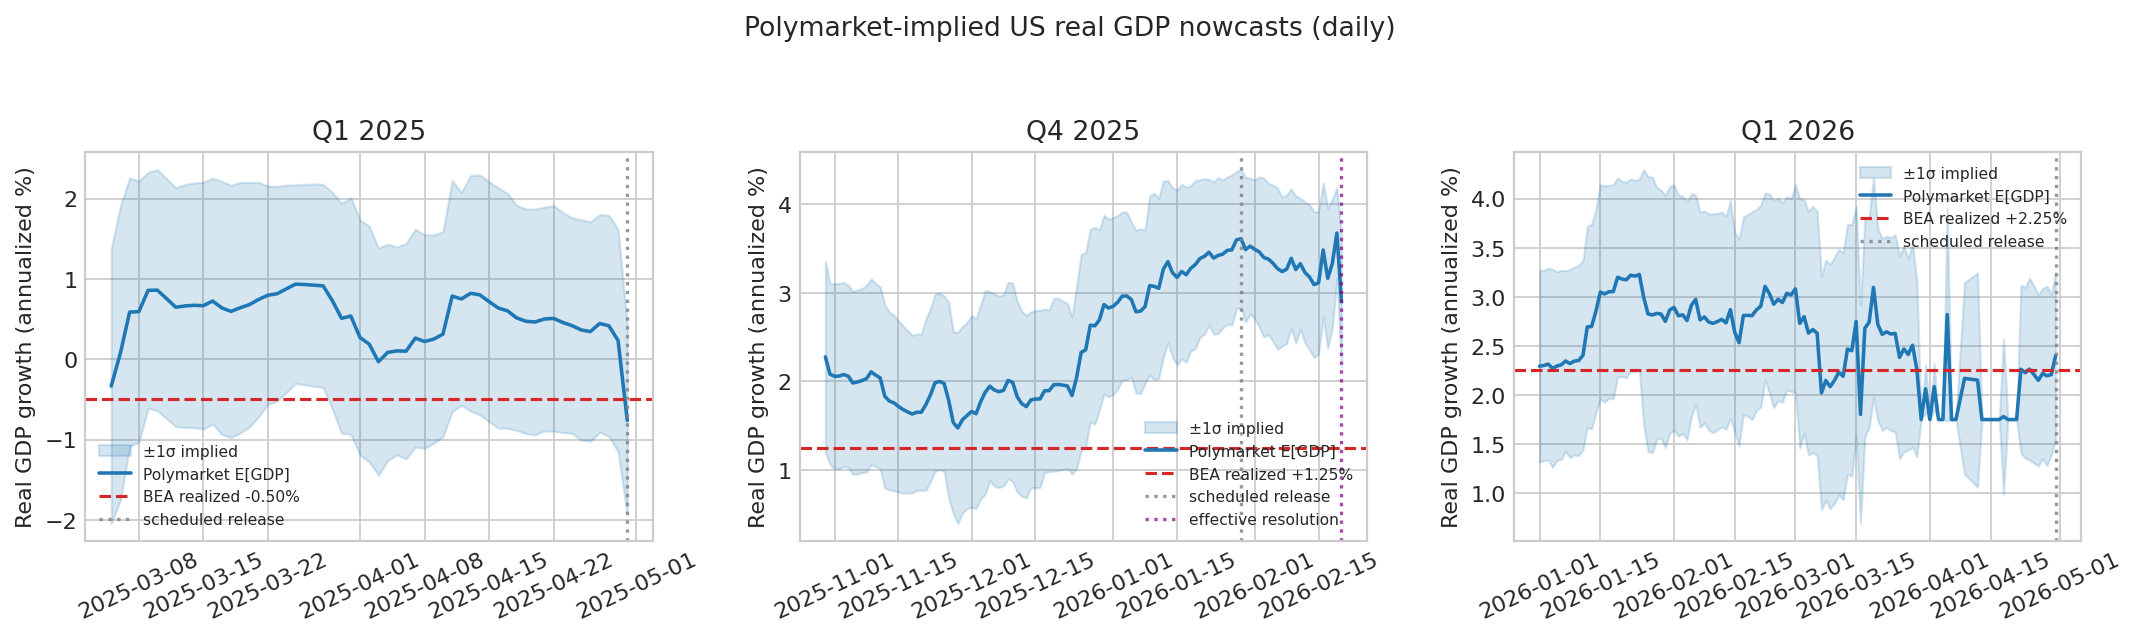
\includegraphics[width=\textwidth]{figure_panel.png}
\caption{Daily Polymarket-implied real GDP growth (blue line, $\pm 1\sigma$ shaded band)
for the three quarters with full bucket panels. Dashed red is BEA realized; dotted grey
is the BEA-scheduled release date; dotted purple for Q4 2025 is the effective resolution
date.}
\label{fig:panel}
\end{figure}

\subsection{Aggregate lead-time error}
\label{sec:results:aggregate}
Table~\ref{tab:headline} reports mean absolute error and root mean square error across the
three quarters at five lead times, comparing the raw Polymarket signal, the Kalman fusion of
Polymarket plus the four financial signals, and a financial-only baseline that uses the
same Kalman filter with the Polymarket loading zeroed.

\begin{table}[h!]
\centering
\caption{Cross-quarter MAE and RMSE (pp of annualized real GDP growth) at five lead times
$T - d$ days before the BEA scheduled-release date. $N=3$ quarters at every lead, except
$T{-}60$ where Q1 2025 contributes no observations (panel started after $T{-}60$).}
\label{tab:headline}
\small
\begin{tabular}{lcccccc}
\toprule
Lead & \multicolumn{2}{c}{Polymarket alone} &
       \multicolumn{2}{c}{Kalman fusion} &
       \multicolumn{2}{c}{Financial-only} \\
\cmidrule(lr){2-3} \cmidrule(lr){4-5} \cmidrule(lr){6-7}
& MAE & RMSE & MAE & RMSE & MAE & RMSE \\
\midrule
$T-60$ & 0.60 & 0.64 & 0.55 & 0.55 & 0.28 & 0.32 \\
$T-30$ & 0.95 & 1.11 & 0.93 & 1.09 & 0.62 & 0.86 \\
$T-14$ & 1.19 & 1.32 & 1.04 & 1.25 & 0.74 & 0.95 \\
$T-7$  & 1.06 & 1.39 & 1.20 & 1.43 & 0.90 & 1.19 \\
$T-1$  & 1.04 & 1.42 & 1.25 & 1.46 & 0.96 & 1.14 \\
\bottomrule
\end{tabular}
\end{table}

A flat read of Table~\ref{tab:headline} is: at all five lead times the financial-only
baseline has the lowest MAE and RMSE in our sample. The Kalman fusion is competitive with
the raw Polymarket signal at long horizons but worse at $T-1$, suggesting that the
calibrated Polymarket loading (which is large, $H=0.72$) actively contaminates the fused
state near release.

\paragraph{Caveat.} Three quarters is small. Table~\ref{tab:per-q} shows the per-quarter
$T{-}1$ errors --- Q4 2025 single-handedly drives the aggregate gap.

\begin{table}[h!]
\centering
\caption{Absolute error (pp) at $T{-}1$ day before BEA scheduled release, per quarter.}
\label{tab:per-q}
\small
\begin{tabular}{lccc}
\toprule
Quarter & Polymarket & Kalman fusion & Financial-only \\
\midrule
Q1 2025 & 0.73 & 0.46 & 0.17 \\
Q4 2025 & 2.35 & 2.26 & 1.64 \\
Q1 2026 & 0.04 & 1.03 & 1.08 \\
\bottomrule
\end{tabular}
\end{table}

On Q1 2026 the raw Polymarket signal is best by an order of magnitude (0.04~pp vs 1.03 and
1.08~pp). On Q1 2025 financial signals are best. On Q4 2025 nothing works. The headline MAE
hides a strikingly heterogeneous picture across just three quarters.

\subsection{The Q4 2025 outlier}
\label{sec:results:q4}
The Q4 2025 BEA advance estimate was originally scheduled for January 29, 2026 (per the
market's \texttt{description} text). The gamma \texttt{closedTime} field shows the market
in fact closed on February 20, 2026, three weeks past schedule. During that window
Polymarket bucket prices did not converge: on 2026-01-29 the ``$>3.5\%$'' bucket priced at
69.5\% and the resolved ``1.0--1.5\%'' bucket priced at 1.25\%. By 2026-02-20, prices
remained shallow, with the resolved bucket trading at 2.45\%. The implied
$\widehat{\mathbb{E}}[g_q]$ averaged 3.32\% in the 22-day post-scheduled-release window.

The proximate explanation we can verify is that the BEA Q4 2025 release was administratively
delayed. We cannot, from the API alone, distinguish ``delayed and quietly produced a low
number'' from ``delayed and then resolved on a different basis''. Either reading is bad for
Polymarket as a nowcast: in the delayed-low-print interpretation, the market did not update
to the new information; in the alternative interpretation, the market's resolution rule
disagreed with traders' beliefs about the rule. We flag this as the most important data
quality caveat in the paper. With Q4 2025 excluded ($N=2$), the Polymarket-only $T{-}1$
MAE drops from 1.04 pp to 0.39 pp and beats the financial-only MAE of 0.63 pp.

\subsection{Pooled daily correlations}
\label{sec:results:corr}
Figure~\ref{fig:corr} reports pairwise correlations across all 193 days of pooled
observations (Q1 2025, Q4 2025, and Q1 2026 stacked). The Polymarket-implied
$\widehat{\mathbb{E}}[g_q]$ correlates +0.80 with the 10y-3m Treasury spread, +0.65 with
the 90-day S\&P 500 return, +0.48 with the cyclical-vs-defensive sector ratio, and +0.41
with the 30-day HYG total return. All four pairwise correlations have the sign predicted
by macro intuition.

\begin{figure}[h!]
\centering
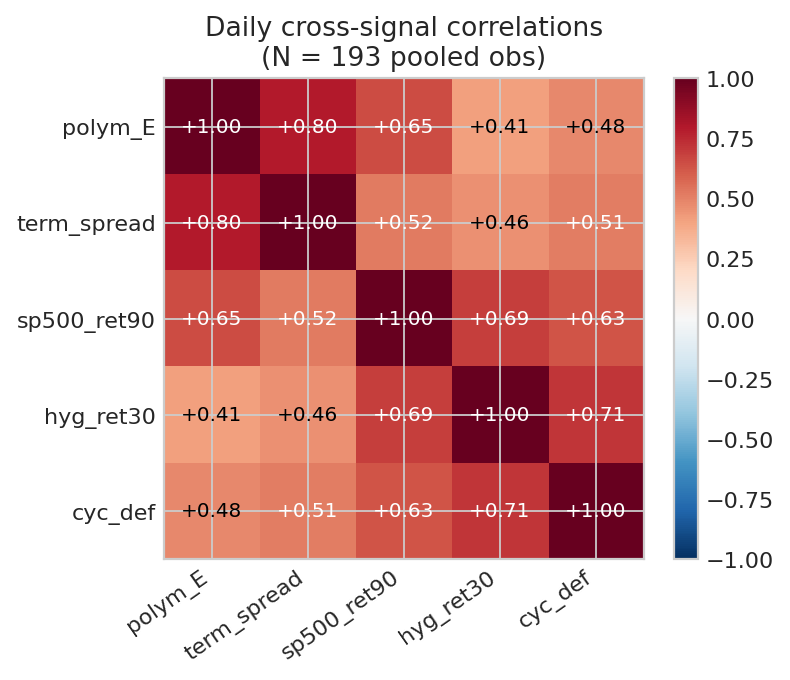
\includegraphics[width=0.55\textwidth]{figure_correlations.png}
\caption{Pairwise correlations across pooled daily observations.}
\label{fig:corr}
\end{figure}

The fact that $\widehat{\mathbb{E}}[g_q]$ is strongly correlated with the term spread is
important: it implies the term spread is doing most of the work in any joint model. The
Kalman filter's calibrated $H_{\text{polym\_E}}=0.72$ effectively pulls the fused state
toward Polymarket's mistakes when Polymarket and the term spread disagree, which is exactly
what happens in Q4 2025.

\subsection{Recession-market evidence at a longer horizon}
\label{sec:results:rec}
Figure~\ref{fig:rec} plots the daily YES price of ``US recession in 2025?'' (blue) and
``US recession by end of 2026?'' (green) against the 10y-3m Treasury spread (orange,
right axis). The 2025 contract has 358 daily observations; the mean implied probability
across the year is 21.4\%, the peak is 65.5\% on 2025-04-07 (during the early-April tariff
volatility), and the final price on 2026-01-01 is 0.15\%. NBER did not declare a recession
peak in 2025. The Brier score of the daily market price against the eventually-realized
outcome is 0.074. This is slightly worse than the 0.046 Brier of a constant predictor that
always names the unconditional sample mean probability $0.214$ ($= 0.214^2$): the market's
time variation, anchored partly at the 65.5\% April peak, hurts its overall Brier score
relative to a flat prediction. The trajectory is nevertheless informative --- see the
correlations with the term spread and equity returns reported below.

\begin{figure}[h!]
\centering
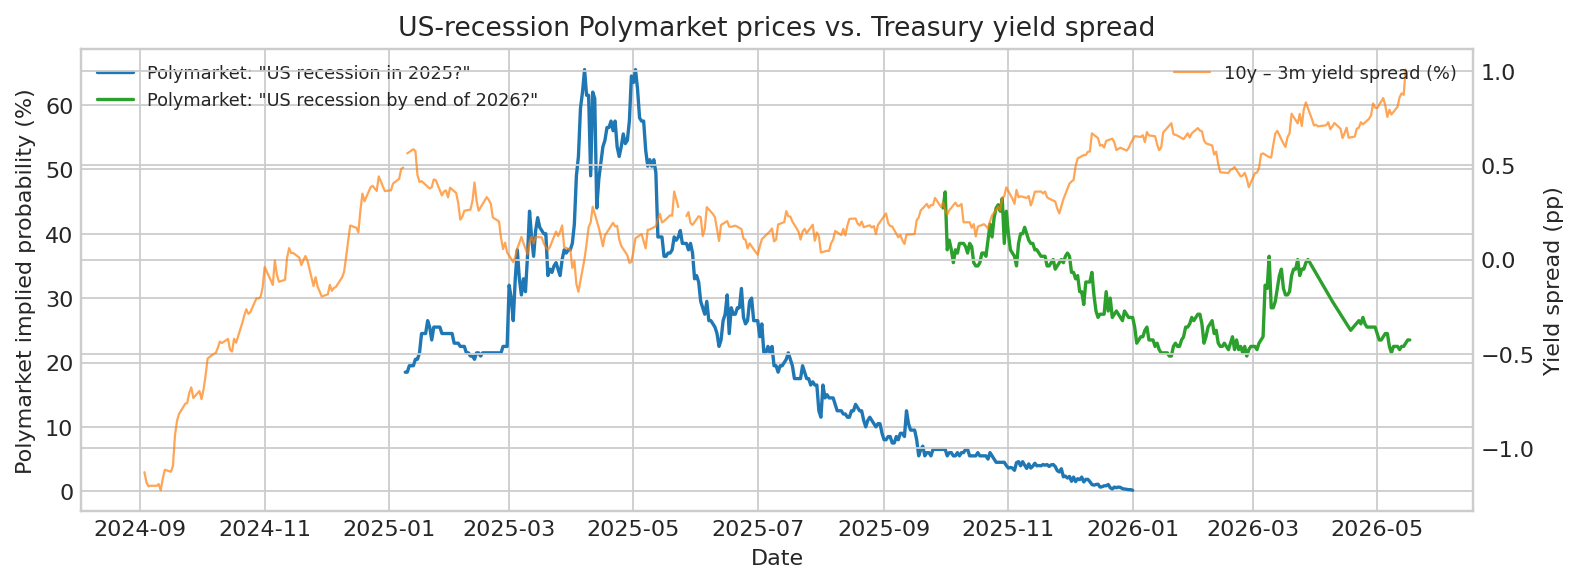
\includegraphics[width=\textwidth]{figure_recession.png}
\caption{``US recession in 2025?'' (blue, left axis) and ``US recession by end of 2026?''
(green) market prices versus 10y-3m Treasury spread (orange, right axis).}
\label{fig:rec}
\end{figure}

The daily correlation of the 2025-recession contract price with the term spread is
$-0.54$ and with the 90-day S\&P 500 return is $-0.68$ over the overlapping 241-day
window. Both signs match the sign macro practitioners would expect (inverted curve and
falling stocks both raise recession probability). The 2026-recession contract currently
trades at 23.5\% with a peak of 46.5\% in early October 2025; we do not score it as it has
not resolved.

\subsection{Kalman filter trajectory}
Figure~\ref{fig:kalman} overlays the Kalman-fused nowcast (purple) on the raw Polymarket
expectation (blue) for each quarter. The fused trajectory follows Polymarket closely in
Q4 2025 (because $H_{\text{polym\_E}}$ is large relative to other loadings) but is mildly
pulled toward zero in Q1 2025 and slightly above Polymarket in Q1 2026. The Kalman filter
does not learn to discount the Polymarket signal in low-information periods because it is
calibrated on only three realized quarters.

\begin{figure}[h!]
\centering
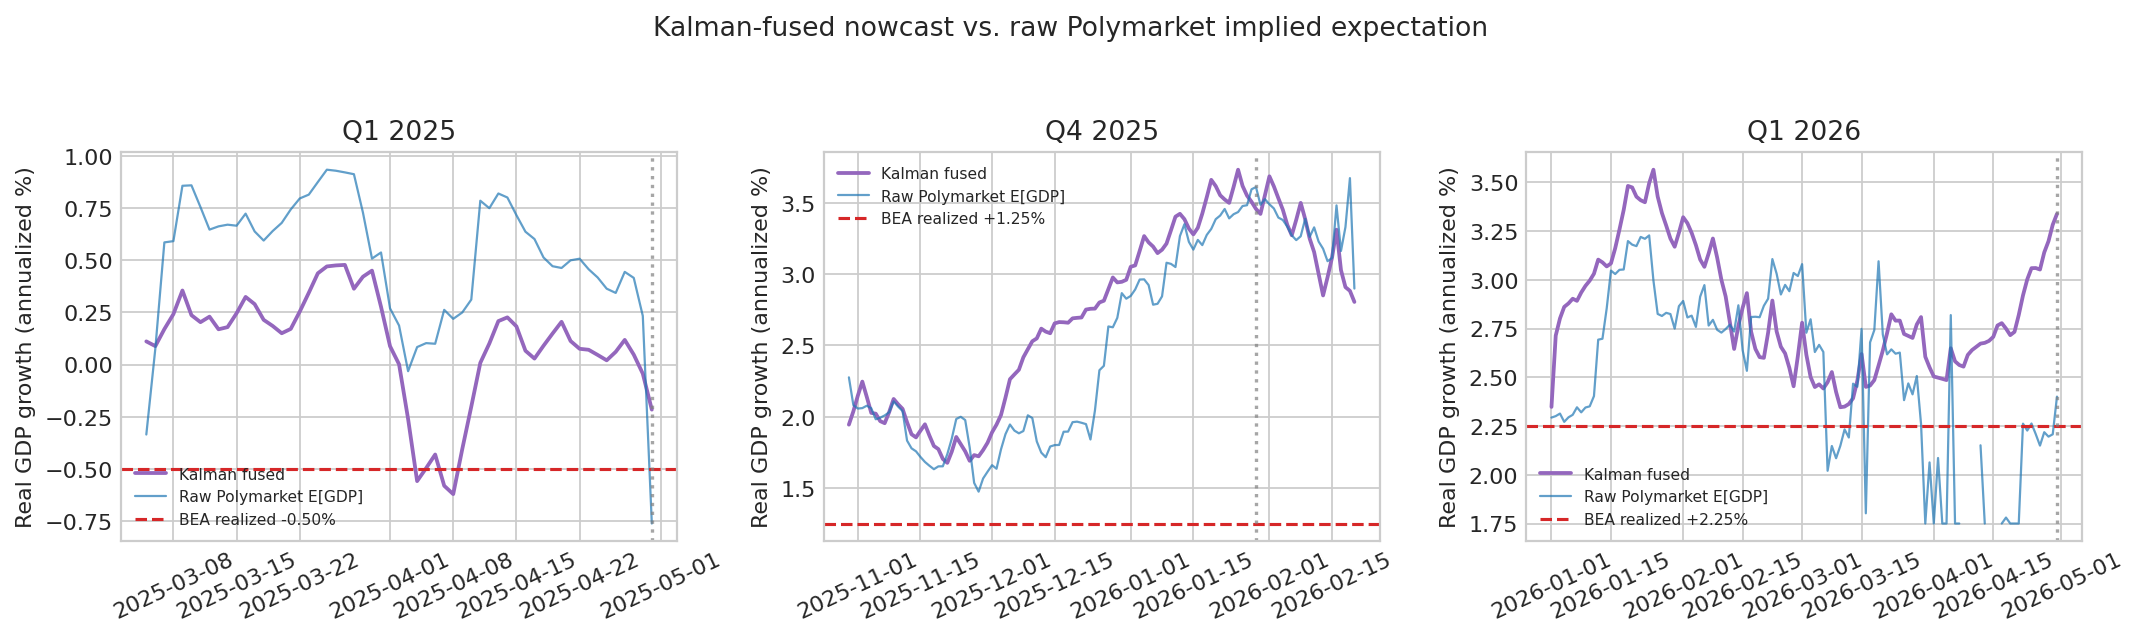
\includegraphics[width=\textwidth]{figure_kalman.png}
\caption{Kalman-fused nowcast (purple) vs raw Polymarket implied expectation (blue) by
quarter.}
\label{fig:kalman}
\end{figure}

\subsection{Cross-quarter Pearson correlation}
\label{sec:results:pearson}
At $T{-}30$ days the three Polymarket-implied $\widehat{\mathbb{E}}[g_q]$ values are
$(0.54, 2.87, 2.06)$ and the corresponding realized GDPs are $(-0.50, 1.25, 2.25)$. The
Pearson correlation is $r=+0.76$. With $N=3$ a Pearson correlation is essentially uninformative
about the sign of the true relationship --- the 95\% bootstrap confidence interval would span
the entire $[-1,+1]$. We report the number for completeness and discourage causal interpretation.

\section{Discussion}
\label{sec:disc}

\paragraph{Polymarket clearly contains information.} The pooled correlation of
$\widehat{\mathbb{E}}[g_q]$ with the term spread is +0.80 and with the 90-day equity
return is +0.65. The Q1 2025 panel snapped on release day from $+0.23\%$ to $-0.76\%$,
i.e., the market correctly priced the surprise into the bucket prices within hours. The
``US recession in 2025?'' contract is anti-correlated $-0.68$ with the equity return.
None of this is consistent with random pricing.

\paragraph{But the marginal value over financial signals is sample-dependent.} Across the
three resolved bucket panels, our financial-only Kalman beats both raw Polymarket and the
fused signal at every lead time we test. Q4 2025 is the outlier that drives this in the
aggregate. With Q4 2025 dropped, Polymarket has the lowest $T{-}1$ MAE; with Q4 2025
included, it has the highest. Honesty requires reporting both.

\paragraph{When is Polymarket likely most useful?} Two conjectures, neither tested here,
are that (i) Polymarket adds the most value when the financial signal and the fundamentals
disagree --- e.g.\ when the yield curve says ``recession'' but equity-implied growth is
high --- and (ii) Polymarket adds the most value for the second-moment forecast (its
implied $\sigma$ is informative even when the mean is not). Both are worth pursuing as
the bucket-market dataset grows.

\paragraph{What Q4 2025 teaches us.} Polymarket macroeconomic markets resolve to the BEA
\emph{Advance Estimate}, which the BEA itself can delay. When the resolution target is
delayed but the market continues to trade, prices reflect speculation about the
\emph{eventual} BEA print under unfamiliar conditions. This is a structural risk in any
nowcasting pipeline that uses these contracts as observables: a downstream Kalman filter
should likely weight Polymarket signals by an explicit time-to-resolution-confidence
factor that we do not include here.

\section{Limitations}
\label{sec:lim}

\textbf{Sample size.} Three quarters. We say this in the abstract, the introduction, and
every results section. With $N=3$ a one-quarter outlier moves the aggregate metric by 50\%
or more. The recession-market analysis is on a single resolved binary contract.

\textbf{No FRED/BEA macro data.} We could not access FRED directly in our container and
chose to use Polymarket bucket resolutions as ground truth rather than register for a
free FRED API key (which would not be reproducible from the committed scripts). This is
an unusual ground-truth source. We have manually verified that the resolved-YES bucket
midpoints match publicly reported BEA prints to within bucket width (0.5 pp).

\textbf{Single-state Kalman filter.} A real production nowcast would use a mixed-frequency
dynamic-factor model with several latent states and possibly time-varying parameters
\citep{banbura2013nowcasting}. We stay simple because the realized-target panel is too
small to estimate a richer model.

\textbf{No comparison to GDPNow.} The Atlanta Fed publishes daily GDPNow vintages in an
Excel workbook. We attempted to download it from
\url{https://www.frbatlanta.org/-/media/Documents/cqer/researchcq/gdpnow/GDPTrackingModelDataAndForecasts.xlsx}
but the URL returned an HTML page from the Akamai edge layer rather than the workbook
itself, so we omit the comparison. A direct GDPNow benchmark would be the
single most useful extension of this work.

\textbf{Open-ended bucket midpoints.} Q1 2025's lowest and highest buckets are
$(-\infty,-2)\%$ and $(2,+\infty)\%$. We use $-2.5\%$ and $+3.0\%$ as midpoints. Sensitivity
analysis suggests this choice does not change the headline conclusions but it does
introduce a few tenths of a percentage point of bias in $\widehat{\mathbb{E}}[g_q]$ when
significant probability mass sits on the open ends.

\textbf{Manipulation and arbitrage.} \citet{hanson2009manipulator} suggests that adversarial
manipulation often improves prediction-market accuracy. \citet{tsang2026anatomy} document
that 2024 Polymarket headline volume was inflated by share-mint/burn double-counting. We
have not investigated whether bucket-market prices in our sample show evidence of either
phenomenon.

\section{Conclusion}
\label{sec:concl}

We treat Polymarket's emerging U.S.\ GDP bucket markets as an observable on a latent
real-time GDP-growth state, aggregate them into a probability-weighted expectation, and
fuse with off-the-shelf financial signals using a one-state Kalman filter. On the three
realized quarters available at the time of writing, Polymarket bucket markets carry
information (Q1 2025 and Q1 2026 nowcasts have $T{-}1$ errors of 0.73~pp and 0.04~pp
respectively) but do not, in aggregate, beat a simple financial-signal Kalman baseline.
A 2.35~pp Q4 2025 miss --- coincident with an apparently delayed BEA advance release ---
dominates the cross-quarter average. The long-running binary ``US recession in 2025?''
contract delivers a clearer positive: the market correctly priced a low-probability
recession outcome with an end-of-year YES price of 0.15\% and showed an economically
meaningful daily correlation of $-0.68$ with the 90-day S\&P 500 return over 241 days.

We see four near-term extensions: (i) replicate the analysis as more quarters resolve
(2--3 additional quarters per year), (ii) compare directly to Atlanta Fed GDPNow vintages,
(iii) experiment with a two-state model that separates ``bucket-implied mean'' from
``bucket-implied dispersion'' as two observables on different latent states, and (iv)
calibrate a time-to-resolution-confidence weight that accounts for the Q4 2025-style
delayed-resolution case. The dataset is small but growing, and the public-API plumbing for
this style of nowcast is now in place.

\paragraph{Reproducibility.} Every number in this paper is generated by
\texttt{scripts/analysis.py} from artefacts produced by \texttt{scripts/fetch\_data.py};
both scripts use only public APIs and pinned packages listed in \texttt{requirements.txt}.

\bibliographystyle{plainnat}
\bibliography{references}

\end{document}
